\documentclass{article}
\title{数値計算入門 — 計算機に数学をさせる}
\author{TeX 図書館}

\begin{document}

\section{この教科書のために — 機械が数学をやるとき}

計算機は\textbf{無限を扱えません}。実数は有限桁の近似で、無限和は打ち切り、微分は差分、積分は足し算です。それでも現代の科学・金融・AI が成り立っているのは、\textbf{誤りの性質を理解した上で、誤りを制御する技術}が発達しているからです。

この教科書では、浮動小数点の誤差、方程式の数値解法(ニュートン法)、数値積分、そして「数値計算が失敗する典型パターン」を学びます。『機械学習入門』で書いた勾配降下法も、実はこの世界の住人です。

\section{浮動小数点数 — 有限の精度で実数を生きる}

計算機の実数は\textbf{浮動小数点数}: 数を「符号 × 仮数 × \(2^{指数}\)」の形で有限桁保持します。これが原因の基本現象:

\begin{lstlisting}[language=Python]
print(0.1 + 0.2)          # 0.30000000000000004
print(0.1 + 0.2 == 0.3)   # False
print(1e16 + 1 == 1e16)   # True (!) — 大きな数は小さな加算を呑む
print(1e308 * 10)         # inf — オーバーフロー
\end{lstlisting}

\begin{itemize}
\item \textbf{丸め誤差}: 0.1 は 2 進では無限小数になるため、有限桁での近似値しか保持できない
\item \textbf{桁あふれ}: \(10^{308}\) を超えると inf に、小さすぎると 0 になる
\item \textbf{カタストロフィー・キャンセル(桁落ち)}: \textbf{近い値同士の減算}で有効数字が消える。1.23456 − 1.23451 = 0.00005 は、両者とも 6 桁有効なのに差は有効 1 桁しかない
\end{itemize}

\begin{quote}
\textbf{【対処の定石】}\ (1) 金額は 10 進の Decimal や整数(円単位)で扱う (2) 近い値の減算は式変形で回避する(例: \(\sqrt{x+\varepsilon} - \sqrt{x}\) は \(\frac{\varepsilon}{\sqrt{x+\varepsilon}+\sqrt{x}}\) に変形)(3) 大小混合の加算は小さい順に足す
\end{quote}

\begin{quote}
\textbf{【演習】}\ 「1 から 10 億までの逆数の和を計算する」際、\texttt{for i in range(1, 10**9)} の順で足すのと逆順(小さい側から)で足すのと、どちらの誤差が少ないか考察せよ。
\end{quote}

\textbf{解答の指針:}\ 逆順(小さい値から)のほうが誤差が少ない。巨大な累積値に微小値を足すと丸めで消えるため、\textbf{小さい数から足し上げて精度を保つ}のが定石です。

\section{ニュートン法 — 接線で方程式を解く}

\(f(x) = 0\) の解を求める最強の定番が\textbf{ニュートン法}です。現在位置での\textbf{接線}と x 軸の交点を次の候補にします:
\[ x_{n+1} = x_n - \frac{f(x_n)}{f'(x_n)} \]

\begin{figure}[h]
\centering
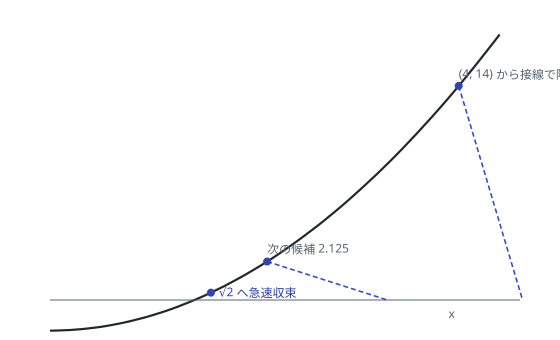
\includegraphics[width=0.75\textwidth]{figures/newton.svg}
\caption{\(f(x) = x^2 - 2\) に対するニュートン法。接線の傾きで次の点へ降りていく。}
\end{figure}

\begin{lstlisting}[language=Python]
def newton(f, df, x0, eps=1e-12, iters=100):
    x = x0
    for i in range(iters):
        x_next = x - f(x) / df(x)
        if abs(x_next - x) < eps:
            return x_next, i + 1
        x = x_next
    return x, iters

root, n = newton(lambda x: x*x - 2, lambda x: 2*x, 4.0)
print(root, n)   # 1.4142135623730951 と数回の反復
\end{lstlisting}

\textbf{収束の速さ}が重要です:\textbf{二分法}は毎回誤差が半分(1 回の反復で有効数字 1 桁)ですが、ニュートン法は解に近づくと\textbf{誤差が 2 乗して消える}(有効数字が\textbf{毎反復倍増})。\(\sqrt{2}\) の計算で反復 4〜5 回で精度 12 桁に達するのはこのためです。

\begin{quote}
\textbf{【注意:失敗パターン】}\ (1) 初期値が悪いと発散・循環する (2) \(f'(x_n) \approx 0\) の点では接線が水平で発散 (3) 複数解がある場合、どの解に落ちるかは初期値次第。実務では二分法と併用して安全域を確保します。
\end{quote}

\begin{quote}
\textbf{【演習】}\ \(\sqrt{2}\) を求める古典的手順「\(x_{n+1} = \frac{1}{2}(x_n + \frac{2}{x_n})\)」が、\(f(x) = x^2 - 2\) に対するニュートン法と一致することを示せ。
\end{quote}

\textbf{解答の指針:}\ ニュートンの式に \(f = x^2-2, f' = 2x\) を代入: \(x - \frac{x^2-2}{2x} = \frac{x}{2} + \frac{1}{x}\)。バビロニア人の手順と 4000 年越しに一致します。

\section{数値積分 — 足し算で面積を}

解析的に積分できない関数(\(e^{-x^2}\) など)の定積分は\textbf{足し算で近似}します。

\subsection{台形公式}

区間を \(n\) 分し、各区間を台形で近似:
\[ \int_a^b f\,dx \approx h\left( \frac{f(a)}{2} + f(x_1) + \cdots + f(x_{n-1}) + \frac{f(b)}{2} \right), \qquad h = \frac{b-a}{n} \]

\begin{lstlisting}[language=Python]
import math

def trapezoid(f, a, b, n):
    h = (b - a) / n
    s = (f(a) + f(b)) / 2
    for i in range(1, n):
        s += f(a + i * h)
    return s * h

for n in [10, 100, 1000]:
    val = trapezoid(lambda x: math.exp(-x*x), 0, 1, n)
    print(n, f"{val:.10f}")
# 分割数を 10 倍にするたび、誤差が約 1/100 になる(2 次収束)
\end{lstlisting}

\begin{quote}
\textbf{【比較:モンテカルロ法】}\ 乱数で面積を推定する方法は誤差が \(1/\sqrt{n}\) 収束——精度 1 桁のためにサンプル 100 倍が必要。台形公式(2 次収束)が使える\textbf{低次元}の問題では決定的に不利です。モンテカルロが強いのは\textbf{高次元}(100 次元積分など)です。
\end{quote}

\begin{quote}
\textbf{【演習】}\ 台形公式の誤差が分割数 \(n\) の 2 乗に反比例する(\(O(1/n^2)\))理由の直感を述べよ。ヒント: 各小区間の近似誤差は曲率 × \(h^3\) で、区間数は \(1/h\) 個。
\end{quote}

\textbf{解答の指針:}\ 各小区間の誤差は幅の 3 乗で消えるが、区間数が幅の逆数で増えるので合計は \(h^3 \times \frac{1}{h} = h^2\)。高次の公式(シンプソン)は曲率補正を入れて \(h^4\) まで改善します。

\section{微分を差分で — 数値微分}

機械学習の勾配計算の基礎もここにあります。前進差分:
\[ f'(x) \approx \frac{f(x + h) - f(x)}{h} \]

\begin{quote}
\textbf{【注意:h の両刃の剣】}\ \(h\) を大きくすると\textbf{打ち切り誤差}(差分と真の微分の乖離)が増え、\(h\) を小さくしすぎると\textbf{丸め誤差}(近い値の減算 = 桁落ち)が増える。\textbf{誤差最小の \(h\) が存在する}(\(10^{-5}\) 程度が目安)——「細かくすれば正確」が\textbf{成り立たない}典型例です。
\end{quote}

改良版の\textbf{中心差分} \(\frac{f(x+h) - f(x-h)}{2h}\) は精度 1 桁上ですが、打ち切り誤差と丸め誤差のトレードオフ構造は同じです。

\begin{quote}
\textbf{【演習】}\ \(f(x) = x^2\) に対し前進差分は \(2x + h\) になることを確かめ、打ち切り誤差が \(h\) に比例することを示せ。
\end{quote}

\textbf{解答の指針:}\ \(\frac{(x+h)^2 - x^2}{h} = 2x + h\)。真値 \(2x\) からのずれはちょうど \(h\)。

\section{数値計算の失敗事例 — 実務の地雷}

\begin{enumerate}
\item \textbf{アリアリ 6 号の爆発(1996)}: 慣性計測の浮動小数点から整数への変換オーバーフローが原因の 1 つ
\item \textbf{ペトリオットミサイルの誤差(1991)}: 0.1 秒を 2 進で近似した累積誤差が 100 時間で約 0.34 秒に成長し迎撃に失敗
\item \textbf{金融の丸め問題}: 利息計算を float で行うと円単位のずれが監査で問題化——\textbf{金額は整数 or Decimal}
\end{enumerate}

\begin{quote}
\textbf{【演習】}\ ペトリオットの失敗を「丸め誤差の蓄積」として説明する数式モデルを書け(ヒント: 0.1 を 2 進有限桁で表した誤差 \(e\) が、100 時間 = 360000 回の加算で積もる)。
\end{quote}

\textbf{解答の指針:}\ 誤差 \(e \approx 10^{-7}\) 秒(0.1 の 2 進近似)が 360000 回積もると \(e \times 360000 \approx 0.03\)〜0.34 秒規模に達しうる。\textbf{小さな誤差でも、繰り返し系では蓄積が破滅的}になりうる。

\section{おわりに — 誤差と付き合う作法}

この教科書の骨格: 浮動小数点の性質と桁落ち(§2)、ニュートン法(§3)、数値積分(§4)、数値微分(§5)、そして実事故(§6)。共通する作法は:

\begin{enumerate}
\item \textbf{誤差の種類を見分ける}: 打ち切り誤差(近似の粗さ)か丸め誤差(有限桁)かで対処が違う
\item \textbf{桁落ちを予感する}: 近い値の減算を見つけたら式変形を考える
\item \textbf{収束の速さを測る}: 分割数を変えて誤差の減り方(次数)を観察する
\item \textbf{繰り返し系の蓄積を恐れる}: 1 回の誤差は小さくても反復で育つ
\end{enumerate}

次の一歩は、Python の NumPy/SciPy(実務の数値計算ライブラリ)、『機械学習入門』の数値最適化、そして『数値計算』の発展である PDE の有限要素法の世界です。

\begin{quote}
\textbf{【総合演習】}
\begin{enumerate}
\item 二分法で \([0, 2]\) の解を精度 \(10^{-6}\) にするには何回の反復が要るか(区間が半分になる)。
\item ニュートン法で \(f(x) = x^2 - 3\) の解を \(x_0 = 2\) から 2 反復求めよ。
\item 台形公式で \(\int_0^1 x^2 dx\) を \(n = 4\) で近似し、真値 \(1/3\) と比較せよ。
\end{enumerate}
\end{quote}

\textbf{解答の指針:}\ 1. \(2^{-n} < 10^{-6}\) より \(n \ge 20\) 回。2. \(x_1 = 2 - 1/4 = 1.75\)、\(x_2 = 1.75 - 0.0625/3.5 \approx 1.7321\)(真値 \(\sqrt{3} \approx 1.73205\))。3. \(h = 0.25\)、値 \(\approx 0.34375\)。真値 0.33333 との差は約 0.0104(\(1/48\)、\(O(h^2)\) に一致)。

\end{document}
